\section{Use-Case 2: Road Warrior} \label{Use-Case 2: Road Warrior}
%Anforderung: Ende-zu-Ende-Erreichbarkeit! Für z.B. Endpoint Scanning
%Gleiches Profil für alle VPN-Konzentratoren

\subsection{Umsetzung: Kerntätigkeiten}

%GeoIP
%Terraform DNS Update
%Bind Split-DNS

In AWS und Azure wurden via Terraform die virtuellen Maschinen VyOS aus den jeweiligen Marketplaces installiert.
Es wurden für die Cloud-Standorte AWS und Azure analog zu Use-Case 1 Templates erstellt, um den Client-VPN-Konzentrator zu installieren. In der Terraform Ressource azurerm\_linux\_virtual\_machine wird das richtige VyOS-Image aus dem Cloud-Marketplace referenziert über source\_image\_reference und lässt dieses installieren. Einige dieser Markeplace-Images bieten verschiedene Support- und Lizenz-Verträge an. Über den \textit{plan \{\}}-Kontext wird der passende Contract ausgewählt (hier: \glqq Standard support\grqq{}). Ähnlich ist für die AWS-Instanz vorzugehen.

\begin{lstlisting}[label=tf-azure-vyos-machine-image,caption=Mit der Terraform-Ressource wird das passende VyOS-Image gesucht und installiert.]
resource "azurerm_linux_virtual_machine"  "azurerm_linux_virtual_machine" {
  name = "vyos-test"
  location = var.rg_location
  resource_group_name = var.rg_name
  admin_username = "vyos"
  size = "Standard_B1s"
  network_interface_ids = [ azurerm_network_interface.azurerm_network_interface.id ]
  os_disk {
    caching = "ReadWrite"
    storage_account_type = "Premium_LRS"
  }
  admin_ssh_key {
    username   = "vyos"
    public_key = file("~/terraform/.cred_mgmt/_push/authorized_keys/id_rsa_automation.pub")
  }
  source_image_reference {
    publisher = "sentriumsl"
    offer = "vyos-1-2-lts-on-azure"
    version = "latest"
    sku = "vyos-1-2-crux"
  }
  plan {
    name = "vyos-1-2-crux"
    product = "vyos-1-2-lts-on-azure"
    publisher = "sentriumsl"
  }
}
\end{lstlisting}

Konfiguriert wurden die virtuellen Maschinen wieder über ein Terraform-Template. Das Public/Private-Schlüsselpaar wurde vorab erstellt, von der pfSense-PKI signiert und mit dem Zertifikat auf dem Terraform-Server gespeichert. Während des Terraform-Deployments wird Private Key und Zertifikat per Terraform Provisioner auf das Zielsystem kopiert. Sie werden in der Config dann via set interfaces openvpn vtun0 tls cert-file / key-file referenziert. In der Praxis sollte darauf verzichtet werden, das Schlüsselmaterial \glqq auf einem anderen System vorzulagern \grqq{}: ein privater Schlüssel nur auf dem Server erzeugt und gespeichert werden, auf dem dieser final genutzt wird. Optimalerweise wäre dies zur Laufzeit der Terraform-Deployments. Zur Vereinfachung des Use-Cases wurde auf diesen Schritt verzichtet. Eine Möglichkeit zur automatisierten Erzeugung von vertrauenswürdigen Zertifikaten ist das Simple Certificate Enrollment Protocol (SCEP)\cite[S.554]{Schmeh2013}.

Für den sich verbindenden VPN-Client sind diverse Konfigurationen hinterlegt: Domain-Name, (interner) Name-Server und Routen, die über den VPN-Konzentrator erreicht werden können.
Weiterhin wird ein MSS-Clamping vorgenommen, um IP-Fragmentierung von TCP-Applikationen möglichst zu verhindern.\\
Das Subnetz, in dem die OpenVPN-Clients terminiert werden, wird wieder dynamisch aus dem IPAM alloziert (s. set interfaces openvpn vtun0 server subnet).

\begin{lstlisting}[label=vpn-c2s-server-config,caption=Terraform Template für VyOS OpenVPN-Server in AWS]
set interfaces openvpn vtun0 openvpn-option "--mssfix 1350"
set interfaces openvpn vtun0 server domain-name 'intern.ba.mungard.de'
set interfaces openvpn vtun0 server name-server '192.168.201.1'
#"dynamic" routes?
set interfaces openvpn vtun0 server push-route '10.32.0.0/16'
set interfaces openvpn vtun0 server push-route '10.33.0.0/16'
set interfaces openvpn vtun0 server push-route '192.168.201.0/24'
set interfaces openvpn vtun0 server subnet ${aws_vpn_clients_subnet}/${aws_vpn_clients_subnet_mask}
set interfaces openvpn vtun0 tls ca-cert-file '/config/auth/BA_CA_2021.crt'
set interfaces openvpn vtun0 tls cert-file '/config/auth/vpn-server-aws.ba.mungard.de.crt'
set interfaces openvpn vtun0 tls dh-file '/config/auth/dh2048.pem'
set interfaces openvpn vtun0 tls key-file '/config/auth/vpn-server-aws.ba.mungard.de.key'
\end{lstlisting}

Die drei Cloud-Standorte wurden in diesem Proof-of-Concept verteilt über verschiedenen Regionen: Dublin (Azure), Frankfurt (AWS), Kiel (Private Cloud). Es werden drei Roadwarrior-Clients simuliert, die ebenso am jeweiligen Standort stehen. Dazu wurden weitere VMs an den Cloud-Standorten hochgefahren: Sie wurden völlig isoliert von dem restlichen Deployment installiert und sich nicht Teil der internen Infrastruktur. Zugang zu internen Ressourcen wird nur über eine erfolgreiche Authentifizierung am VPN-Konzentrator gewährleistet.

\begin{lstlisting}[label=ext-ip-addr-roadwarrior,caption=Der simulierte Roadwarrior-Client ist nicht Teil der Netzwerke 10.32.0.0/16 bzw. 10.33.0.0/16]
ubuntu@vpn-client-azure:~$ ip -brief -4 address show | grep -v lo
eth0             UP             10.42.0.4/24
\end{lstlisting}

Internet-Traffic ist möglich, Zugriff auf interne Ressourcen ist nicht möglich: 192.168.201.1 ist eine IP-Adresse der Private Cloud.

\begin{lstlisting}[label=internet-access-roadwarrior,caption=Der Roadwarrior-Client kann auf das Internet zugreifen, jedoch nicht auf interne Ressourcen ohne VPN-Einwahl]
#Internet-Traffic
ubuntu@vpn-client-azure:~$ ping -c 1 8.8.8.8
PING 8.8.8.8 (8.8.8.8) 56(84) bytes of data.
64 bytes from 8.8.8.8: icmp_seq=1 ttl=112 time=0.987 ms

--- 8.8.8.8 ping statistics ---
1 packets transmitted, 1 received, 0% packet loss, time 0ms
rtt min/avg/max/mdev = 0.987/0.987/0.987/0.000 ms

#Interne Adresse ist nicht erreichbar 
ubuntu@vpn-client-azure:~$ ping -c 1 192.168.201.1
PING 192.168.201.1 (192.168.201.1) 56(84) bytes of data.

--- 192.168.201.1 ping statistics ---
1 packets transmitted, 0 received, 100% packet loss, time 0ms
\end{lstlisting}

Die MaxMind GeoIP-Datenbank wurde auf dem DNS-Server installiert und in der Bind-Konfiguration referenziert:

\begin{lstlisting}[label=bind-geoip-directory,caption=.]
$ grep -E 'options|geoip-directory|^};' < named.conf.options
options {
        geoip-directory "/usr/share/GeoIP";
};
\end{lstlisting}

Dadurch wurde ermöglicht, GeoIP-Daten in einer Access Control List (ACL) zu nutzen und verschiedene Fälle zu definieren. Die ACL heißt in diesem Falle \glqq dublin\grqq{} und erlaubt Zugriffe aus der Stadt Dublin bzw. Zugriff für den TSIG-Key db-vpn.ba.mungard.de. Dieser Key wird benötigt, um Zonen-Updates machen zu können und ist im entsprechenden Terraform-Modul hinterlegt.

\begin{lstlisting}[label=acl-geoip-bind,caption=.]
acl "dublin" {
        geoip city Dublin;
        key "db-vpn.ba.mungard.de.";
};
\end{lstlisting}

Weiterhin existiert ein \textit{View} \glqq Dublin\grqq{}, in dem die ACL und Zonen-Daten zusammengeführt werden. Mit \textit{allow-update} werden Zonen-Updates explizit und ausschließlich für genannten TSIG-Key erlaubt.

\begin{lstlisting}[label=view-geoip-bind,caption=.]
view "dublin" {
        match-clients { dublin; };
        zone "ba.mungard.de" {
                type master;
                file "/etc/bind/ba_zones/db.geo.ba.mungard.de-dublin";
                allow-update { key "db-vpn.ba.mungard.de."; };
        };
};
\end{lstlisting}

In der Zonen-Datei für Dublin befindet sich vor Terraform-Deployment nur ein A-Record \textit{default-vpn}. Dies ist der A-Record, der als Fallback dient. Gemäß Evaluationskriterien muss ein Roadwarrior-Client auf die Private Cloud zurückfallen, wenn bisher kein Deployment stattgefunden hat. Die öffentlich auflösbare Zone lautet \textit{ba.mungard.de}.

\begin{lstlisting}[label=zone-dublin-before-deployment,caption=Die Zone ba.mungard.de vor dem Terraform-Deployment.]
$ grep -A1 "ORIGIN ba.mungard.de" < /etc/bind/ba_zones/db.geo.ba.mungard.de-dublin
$ORIGIN ba.mungard.de.
default-vpn             A       195.244.254.197
\end{lstlisting}

Die Konfigurationen für Frankfurter und Kieler Clients wurden analog vollzogen. Dies gilt ebenso für das interne DNS. Allerdings wird hier kein GeoIP genutzt, sondern anhand der Absender-IP-Adresse wird eine ACL (hier \glqq dublin-internal\grqq{}) \textit{getroffen}. Auch die internen Zonen sind durch Terraform via DNS UPDATE editierbar (key \glqq db-vpn-internal.ba.mungard.de.\grqq{}).

\begin{lstlisting}[label=view-internal-bind,caption=Absender-IPs aus dem Netzwerk 10.32.0.0/16 treffen die ACL dublin-internal.]
acl "dublin-internal" {
        10.32.0.0/16;
        key "db-vpn-internal.ba.mungard.de.";
};
\end{lstlisting}

Weiterhin gibt es eine ACL \glqq match-all\grqq{}, welche für anfragende Clients vorgesehen ist, die nicht per GeoIP identifiziert werden. Durch das Netzwerk 0.0.0.0/0 treffen die ACL alle restlichen Teilnehmer des Internets.

\begin{lstlisting}[label=view-matchall-bind,caption=.]
acl "match-all" {
        0.0.0.0/0;
        key "all-vpn.ba.mungard.de.";
};
\end{lstlisting}


Aus Sicht des Terraform-Moduls muss erstens ein Provider \textit{pro} TSIG-Key konfiguriert werden, weiterhin. Der server-Parameter konfiguriert den Nameserver, der per DNS UPDATE editiert werden soll. Außerdem ist das Pre-Shared-Secret (TSIG-Key) hinterlegt. Es wird für die Domain vpn.ba.mungard.de die IP-Adresse des VPN-Konzentrators in Dublin (Azure) eingetragen, welche dynamisch zur Laufzeit entsteht (\textit{var.dublin\_ip}).

\begin{lstlisting}[label=tf-provider-dns,caption=.]
provider "dns" {
        alias = "dns-dublin"
        update {
                server        = "192.168.200.29"
                key_name      = "db-vpn.ba.mungard.de."
                key_algorithm = "hmac-sha256"
                //Key für die Dokumentation aus Sicherheitsgründen geändert
                key_secret    = "9jzMaHwILwTzx9b/Ws8RAfBwC+eJpjOI2hEmAgCjV/4="
        }
}
resource "dns_a_record_set" "vpn-dublin" {
        provider = dns.dns-dublin
        zone = "ba.mungard.de."
        name = "vpn"
        addresses = [ var.dublin_ip ]
        ttl = 15
}
\end{lstlisting}

Nach dem Terraform-Deployment kann man sich per \textit{rndc dumpdb -zones} alle Views ausgeben lassen (hier eingefiltert auf die relevantesten Einträge der Views \glqq dublin\grqq{} und \glqq match-all\grqq{}). Man sieht, dass in beiden Views für die Domain default-vpn.ba.mungard.de die gleiche IP (\glqq Fallback\grqq{}) zurückgegegeben. Für Domain vpn.ba.mungard.de wird ist im View \glqq dublin\grqq{} nur eine Azure-IP sichtbar, während im View \glqq match-all\grqq{} IPs aller VPN-Konzentratoren des Deployments auftreten.

\begin{lstlisting}[label=tf-provider-dns,caption=.]
$ grep -E -A12 'Start view (dublin|match-all)$' < /var/cache/bind/named_dump.db | grep -Ev '(client|SOA|NS|nu|^;$)'
; Start view dublin
; Zone dump of 'ba.mungard.de/IN/dublin'
default-vpn.ba.mungard.de.                    15 IN A           195.244.254.197
vpn.ba.mungard.de.                            15 IN A           137.116.237.246
; Start view nu
--
; Start view match-all
; Zone dump of 'ba.mungard.de/IN/match-all'
default-vpn.ba.mungard.de.                    15 IN A           195.244.254.197
vpn.ba.mungard.de.                            15 IN A           18.197.9.208
vpn.ba.mungard.de.                            15 IN A           137.116.237.246
vpn.ba.mungard.de.                            15 IN A           195.244.254.197
\end{lstlisting}

Zusammenfassend die GeoIP-Konfiguration als Entscheidungsbaum.
\begin{figure}[h]
  \centering
  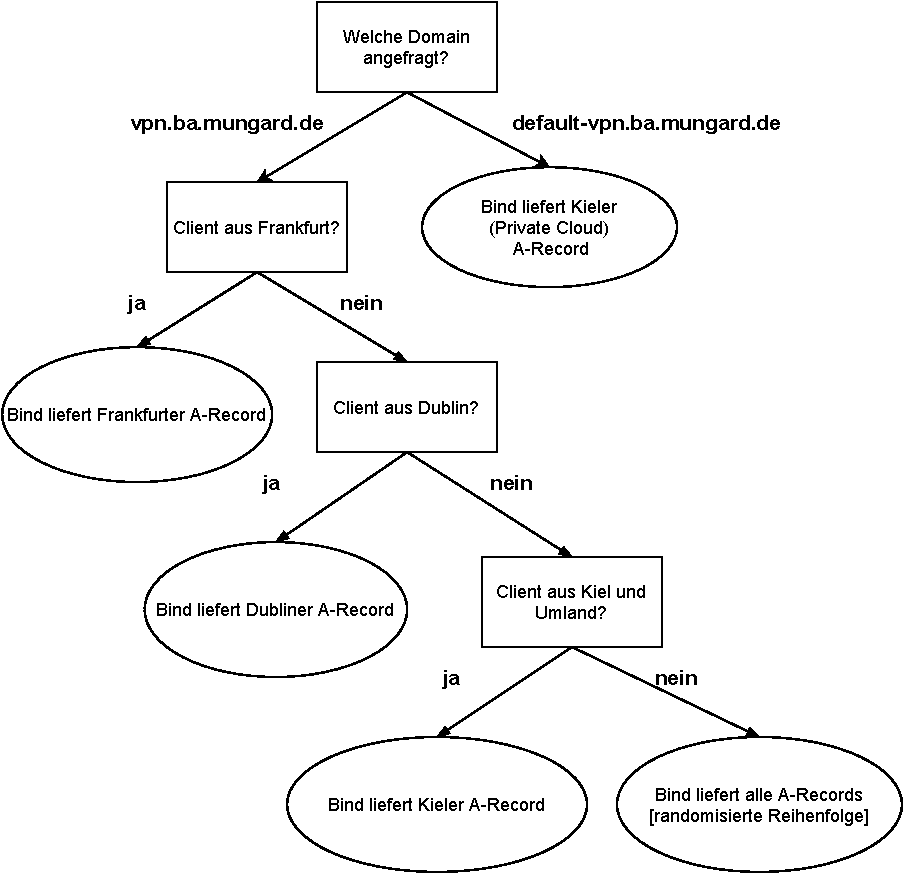
\includegraphics{Figures/entscheidungsbaum_bind_geoip.pdf}
  \caption{Entscheidungsbaum: GeoIP}
  \label{grafik:Use-Case_2_Entscheidungsbaum_GeoIP}
\end{figure}\FloatBarrier

Weiterhin ein exemplarischer Zone-Dump für einen internen Client, welcher über Dublin verbunden ist. Die interne Zone ist intern.ba.mungard.de. Alle Cloud-Standorte nutzen den gleichen Name-Server (ns1.intern.ba.mungard.de), welcher in der Private Cloud vorhanden ist.\\

\begin{lstlisting}[label=tf-provider-dns,caption=.]
$ grep -E -A10 'Start view dublin-internal' < /var/cache/bind/named_dump.db | grep -Ev '(client|SOA|NS|^;$)'
; Start view dublin-internal
; Zone dump of 'intern.ba.mungard.de/IN/dublin-internal'
ns1.intern.ba.mungard.de.                     15 IN A           192.168.201.1
www.intern.ba.mungard.de.                     15 IN A           10.32.0.4
\end{lstlisting}

%Deployment Webserver
Es wurde eine Ubuntu-VM pro Standort (hier Azure in Dublin) via Terraform deployed. Per remote-exec provisioner wird das Apache2-Paket installiert und die Default-HTML-Seite (\glqq It works!\grqq{}) per \textit{sed} manipuliert. Damit soll der Standort verdeutlicht werden, von dem die HTML-Seite ausgeliefert wurde. Analoge Konfiguration hat für den Standort AWS in Frankfurt stattgefunden.

\begin{lstlisting}[label=tf-provider-dns,caption=.]
resource "null_resource" "www_config" {
        depends_on = [ azurerm_virtual_machine.azurerm_virtual_machine ]
        connection {
                type = "ssh"
                host = azurerm_network_interface.azurerm_network_interface.private_ip_address
                user = "ubuntu"
                private_key = file(var.private_key_file)
        }

        provisioner "remote-exec" {
                inline = [ "sudo http_proxy=\"http://192.168.201.1:8080\" apt update",
                           "sudo http_proxy=\"http://192.168.201.1:8080\" apt install -y apache2",
                           "sudo sed -i 's/It works!/It works! @Azure Cloud (Location: \"North Europe - Dublin\")/' /var/www/html/index.html" ]
        }
}
\end{lstlisting}

% Binärer Entscheidungsbaum OpenVPN

Die OpenVPN Client-Konfigurationen wurden vor Terraform-Deployment bereits \textit{inline} in einer Textdatei vorbereitet. Auch hier gilt analog zur Server-Konfiguration, dass Schlüsselmaterial optimalerweise erst zur Laufzeit erstellt wird. Zertifikate und privater Schlüssel wurden im folgenden Beispiel gefiltert. Von zentraler Bedeutung sind Zeilen 2 und 3: Durch mehrfache Angabe einer remote-Direktive kann ein Fallback auf default-vpn.ba.mungard.de stattfinden, sollte vpn.ba.mungard.de nicht auflösbar sein.\\
Dies gilt für den Fall, falls das Deployment noch nicht stattgefunden hat und der Client nicht in der Nähe von Kiel ist, um per GeoIP-ACL Zugriff auf die Auflösung von vpn.ba.mungard.de erhält. Per pullfilter ignore redirect-gateway wird verhindert, dass ein Default Gateway über den Tunnel signalisiert wird: Alle weiteren, bekannten Routen kommen über die OpenVPN-Server-Konfiguration (s. oben).

\begin{lstlisting}[label=ovpn-client-conf,caption=.]
$ grep -B100 '<ca>' ~/terraform/.cred_mgmt/_push/openvpn/azure_client/config.ovpn | grep -v '<ca>'
remote vpn.ba.mungard.de 61231
remote default-vpn.ba.mungard.de 61231
port 0
pull-filter ignore redirect-gateway
cipher aes-256-cbc
client
dev tun
resolv-retry infinite
remote-cert-tls server
verb 3
persist-tun
\end{lstlisting}

Dieser simple Entscheidungsbaum soll den wichtigen Aspekt des \glqq DNS-Fallbacks\grqq{} nochmals verdeutlichen.

\begin{figure}[h]
  \centering
  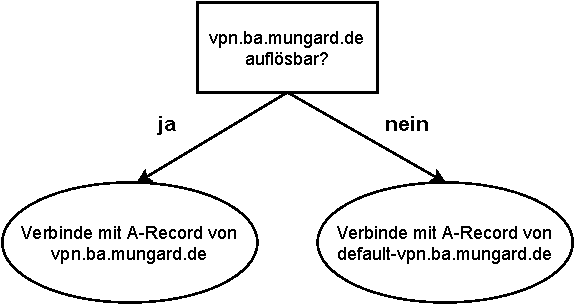
\includegraphics{Figures/entscheidungsbaum_openvpn_config.pdf}
  \caption{Entscheidungsbaum: OpenVPN-Verbindungsversuch}
  \label{grafik:Use-Case_2_Entscheidungsbaum_OpenVPN}
\end{figure}\FloatBarrier

\subsection{Probleme und Lösungsfindung}
%VyOS Images finden? az CLI, AWS Suche funktioniert nicht
%Die richtigen Images für die VyOS-Maschinen der jeweiligen Cloud-Marketplaces auf Terraform zu übertragen, erwies sich als nicht trivial...
%Lizenzen muss zugestimmt werden -> manuell!!!!

%Statische Routen innerhalb VPC nicht more specific -> Transit Gateway
%Import von Remote State, um Azure VPN Gateway zu verkürzen... Eigentlich ziemlich coole Idee von mir... :)
%mmdb.py damit man nicht "blind" ist...

\textbf{\underline{Beschleunigung des Deployments}}\\
Wie bereits in Use-Case 1 (Lösungsfindung...) geschildert, benötigt das Azure VPN Gateway viel Zeit für die Erstellung. Da Use-Case 2 direkt auf diesem Use-Case aufsetzt, hätte das ebenso eine lange Deployment-Zeit nach sich gezogen. So war ursprünglich war die Idee, den Programmcode aus Use-Case 1 zu klonen und um die Infrastruktur-Komponenten aus Use-Case 2 zu ergänzen. Somit hätte sich die Deployment Zeit $t_{gesamt}$ aus den jeweiligen Deployment-Zeiten der Infrastrukturen aus Use-Case 1 und Use-Case 2 zusammengesetzt:\\
$t_{gesamt} = t_{Infrastruktur_{U1}} + t_{Infrastruktur_{U2}}$

Somit kam die Frage auf, ob man das Deployment beschleunigen könnte. Da in Use-Case 2 viele Tests und Änderungen gemacht wurden, musste oftmals komplett re-deployet werden, Deployment-Zeiten von bis zu anderthalb Stunden (s. Probleme Redeployment) mit sich bringen kann.\\
Dieses Problem konnte mit terraform\_remote\_state zumindest abgemildert werden. So wurde Use-Case 1 als vorhanden angenommen und die Infrastruktur aus Use-Case 2 lediglich hinzugefügt. Der \textit{state import} findet in der Datei main.tf von Use-Case 2 statt und referenziert die Datei terraform.tfstate aus Use-Case 1.

\begin{lstlisting}[label=tf-remote-state-import,caption=.]
$ grep -A6 \"terraform_remote_state\" < main.tf
data "terraform_remote_state" "base_deployment" {
  backend = "local"
  config = {
    path = "../use_case_1/terraform.tfstate"
  }
}
\end{lstlisting}

Der Remote-State-Import dauert einen kurzen Moment, wird aber in der folgenden Betrachtung vernachlässigt.
Effektiv ist die Laufzeit des Deployments damit:\\
$t_{gesamt} = t_{Infrastruktur_{U2}}$

Im Allgemeinen hat sich dieser \glqq Teile-und-herrsche\grqq{}-Ansatz im Zusammenspiel mit Terraform als sehr hilfreich erwiesen, um Konsistenz-Probleme der asynchronen Cloud-APIs während der Deployment-Phase zu verringern \cite[S.183-184]{Brikman2019}. Probleme während des Deployments entstanden v.a. dann, wenn \glqq zu viele\grqq{} Abhängigkeiten der Infrastruktur-Komponenten im Spiel waren. Für die Verschaltung von \textit{gesplitteten} Terraform-Deployments eignet sich das Werkzeug Terragrunt \cite[S.98]{Brikman2019}.

%https://web.archive.org/web/20210123233358/https://docs.aws.amazon.com/vpc/latest/userguide/vpc-ug.pdf Seite 230
\textbf{\underline{More-Specific Route nicht möglich in VPC Routing-Tabelle}}\\


\textbf{\underline{Untersuchung von GeoIP-Daten}}\\
%https://linux.die.net/man/1/file
Die GeoIP-Datenbank liegt als Binärformat auf der Festplatte.

\begin{lstlisting}[label=tf-remote-state-import,caption=.]
$ file /usr/share/GeoIP/GeoLite2-City.mmdb
/usr/share/GeoIP/GeoLite2-City.mmdb: data
\end{lstlisting}

%https://web.archive.org/web/20201110053320/https://github.com/maxmind/MaxMind-DB-Reader-python
%https://bind9.readthedocs.io/en/latest/security.html?highlight=geoip#access-control-lists
Die Datensätze mussten \glqq sichtbar\grqq{} gemacht werden, um eine Idee zu bekommen, welche Spezifizierer genutzt werden können, um die DNS-Auflösung in regionaler Abhängigkeit umzusetzen. Weiterhin war nicht sichergestellt, welche Qualität die Datensätze aufweisen. Um dies zu testen, wurde kurze Python-Skript \textit{mmdb.py} geschrieben und das Modul \textit{maxminddb} des GeoIP-Anbieters MaxMind eingebunden. Per \textit{pretty print} konnten die entsprechenden Datensätze für eine IP-Adresse ausgegeben werden.

\begin{lstlisting}[label=mmdb-code-example,caption=.]
#!/usr/bin/python3
import maxminddb
import sys
import pprint
#aehnliche Code-Teile uebersprungen
print("++++++++++++++++++++ CITY INFO +++++++++++++++++++\n")
with maxminddb.open_database('/usr/share/GeoIP/GeoLite2-City.mmdb') as reader:
    pprint.pprint(reader.get(sys.argv[1]))
print("++++++++++++++++++++ CITY INFO +++++++++++++++++++\n")
\end{lstlisting}

Anbei eine Beispielausgabe für eine IP-Adresse der Fachhochschule Kiel.

\begin{lstlisting}[label=mmdb-show-ip,caption=.]
$ dig +short fh-kiel.de A
149.222.20.63

\

$ mmdb.py 149.222.20.63
++++++++++++++++++++ ASN INFO ++++++++++++++++++++

{'autonomous_system_number': 680,
 'autonomous_system_organization': 'Verein zur Foerderung eines Deutschen '
                                   'Forschungsnetzes e.V.'}
++++++++++++++++++++ ASN INFO ++++++++++++++++++++
[...]
++++++++++++++++++++ CITY INFO +++++++++++++++++++

{'city': {'geoname_id': 2891122,
          'names': {'de': 'Kiel',
                    'en': 'Kiel',
                    [...]
[...]
 'location': {'accuracy_radius': 20,
              'latitude': 54.3258,
              'longitude': 10.1379,
              'time_zone': 'Europe/Berlin'},
 'postal': {'code': '24149'},
[...]
++++++++++++++++++++ CITY INFO +++++++++++++++++++
\end{lstlisting}

Insgesamt erwiesen sich die Datensätze als sehr brauchbar und akkurat. Per cron-Job wird die Datenbank wöchentlich aktualisiert.

\subsection{Evaluation}

%dig für "next hop"n
%whois Daten